\documentclass[14pt,margin=0.5in,innermargin=0in,blockverticalspace=-0.1in,colspace=-1.2cm]{tikzposter}
\geometry{paperwidth=841mm,paperheight=594mm}
\usepackage[utf8]{inputenc}
\usepackage{lmodern}
\usepackage{anyfontsize}
\usepackage{csquotes}
\usepackage{amsmath}
\usepackage{amsfonts}
\usepackage{amsthm}
\usepackage{amssymb}
\usepackage{mathrsfs}
\usepackage{graphicx}
\usepackage{adjustbox}
\usepackage{enumitem}
\usepackage{xcolor}
\usepackage[backend=biber,style=numeric,sorting=none]{biblatex}
\usepackage{durham-theme}
\usepackage{mwe} % for placeholder images
\usepackage{tcolorbox}
\usepackage{multicol}

\usepackage{caption}
\captionsetup[figure]{font=Large,labelfont=bf}

\addbibresource{references.bib}

% set theme parameters
\tikzposterlatexaffectionproofoff
\usetheme{DurhamTheme}
\usecolorstyle{DurhamStyle}

\usepackage[scaled]{helvet}
\renewcommand\familydefault{\sfdefault} 
\renewcommand{\vec}[1]{\bm{#1}}
\newcommand{\Tr}{\text{Tr}}
\usepackage[T1]{fontenc}

\usepackage{enumitem}
\setitemize{noitemsep,topsep=0pt,parsep=0pt,partopsep=0pt}

\title{Megapixel Image Generation with Step-unrolled Denoising Autoencoders}
\author{\textbf{Alex F. McKinney}, \textbf{Chris G. Willcocks}
}
\institute{ }
%\titlegraphic{
\includegraphics[width=0.16\linewidth]{durham-logo.png}}

% begin document
\begin{document}
\maketitle

\centering
\block{}
{
    \vspace{-2.5cm}
    \centering
    \begin{tikzfigure}
        \includegraphics[width=1.0\linewidth]{samples.png}
    \end{tikzfigure}
    \captionof{figure}{
            \centering
            Samples from our FFHQ1024 model. Resulting samples are diverse and
            of high-fidelity. \textbf{Each $\bf 1024 \times 1024$ sample was
            generated in two seconds} on a consumer-grade GPU (GTX 1080Ti), in
            contrast to existing approaches at this resolution, which take
            minutes to generate. To our knowledge, this is the fastest sampling,
            non-adversarial generative framework at this resolution.
        }
    \vspace{0.5cm}
    \begin{scope}[line width=\titlelinewidth,]
    \draw[color=colorOne!30!colorOne,round cap-round cap]
    (\titleposleft,0)--(100,0);
    \end{scope}
}

\begin{columns}

    \column{0.3}
    \block{}{
        \vspace{-1cm}
        \begin{tcolorbox}[boxsep=0pt,top=0cm,bottom=0.2cm,adjusted title={\huge\bf
            Background},colbacktitle=colorOne]
        \begin{tikzfigure}
            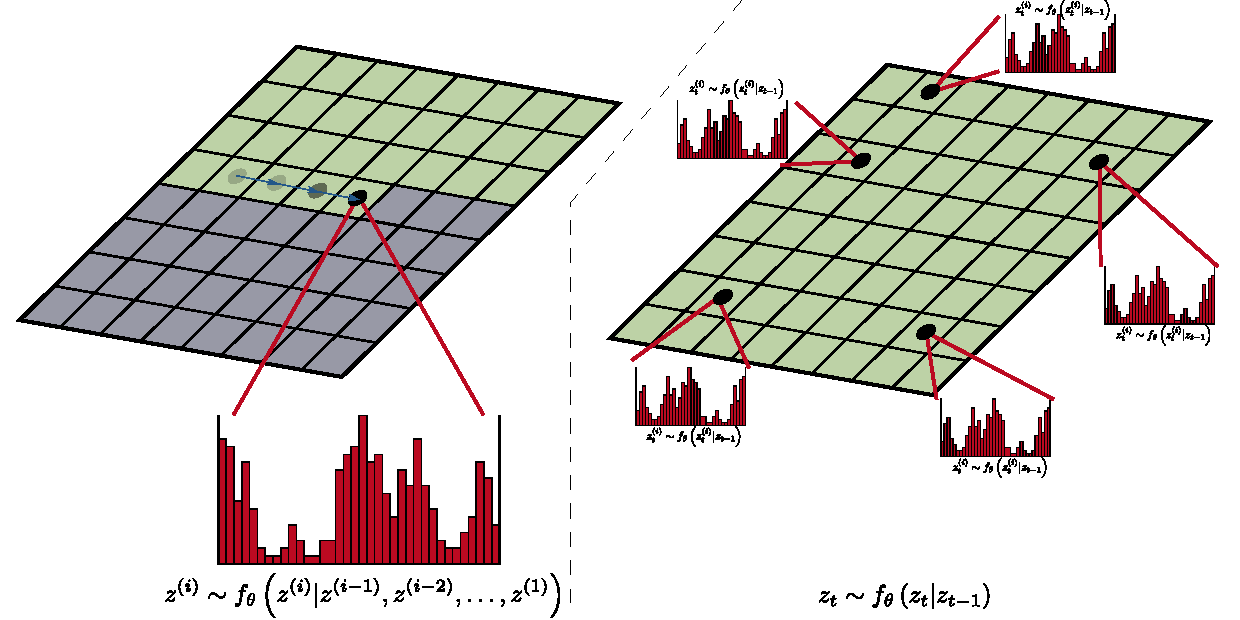
\includegraphics[width=1.0\linewidth]{AR-NAR.pdf}
        \end{tikzfigure}
        \vspace{-0.5cm}
        %\captionof{figure}{
                %Autoregressive sampling (left) is defined in terms of the
                %probabilistic chain rule, so sampling is done iteratively with
                %complexity $\mathcal{O}(n)$. Non-autoregressive sampling (right)
                %can sample an arbitrary number of elements in parallel, so
                %number of steps does not scale with input size. It can also use
                %the full context available to it, resulting in better quality
                %samples and flexible inpainting. However, existing NAR methods
                %still typically require many network evaluations to produce
                %meaningful samples.
            %}

        {
            \Large
            \begin{itemize}
                \item[--] \textbf{Autoregressive (AR)} sampling (left) is defined by the
                    probabilistic chain rule. This means sampling is done
                    iteratively with complexity $\mathcal{O}(n)$.
                \item[--] \textbf{Non-autoregressive (NAR)} sampling (right) samples an arbitrary
                    number of elements in parallel and does not scale with input
                    size $n$, but may still require thousands of iterations.
                \item[--] AR sampling is \textbf{limited to using past context}, whereas NAR
                    uses \textbf{all context available to it}.
            \end{itemize}
        }
        
        \vspace{0.0cm}

        \begin{tikzfigure}
            \includegraphics[width=0.99\linewidth]{recon.pdf}
        \end{tikzfigure}
        \vspace{-1.0cm}
        %\captionof{figure}{
                %VQ-GAN is used to reduce computational requirements for training
                %and sampling of generative models by acting as a compression
                %model. VQ-GAN does not always faithfully reproduce the input
                %image, though outputs are perceptually valid. For example, left
                %shows a change in eye colour and the concealment of a piercing
                %by adjusting hair position. Middle has its hair texture changed.
                %Right has piercings removed and text corruption.
            %}

        {
            \Large
            \begin{itemize}
                \item[--] \textbf{VQ-GAN} is used to reduce computational requirements in
                    generative models by compressing the input.
                \item[--] It offers a higher compression rate than prior work, but
                    does not always faithfully reconstruct the input, for
                    example the left changes the eye colour, and the right has
                    piercings removed.
            \end{itemize}
        }
            
        \end{tcolorbox}
    }
    
    \column{0.4}
    \block{}{
        \vspace{-1cm}
        \begin{tcolorbox}[boxsep=0pt,top=0cm,bottom=0.6cm,adjusted title={\huge\bf Proposed Method},colbacktitle=colorOne]
        \begin{tikzfigure}
            \includegraphics[width=0.99\linewidth]{overall.pdf}
        \end{tikzfigure}
        \vspace{-0.5cm}
        %\captionof{figure}{
                %An overview of the SUNDAE training and sampling of discrete
                %latent representations. Above the dashed line represents the
                %process for training, whereas below the dotted line represents
                %the sampling process. The training process begins by sampling
                %$\mathbf{z} \sim \mathcal{L}$ and then sampling from the
                %corruption distribution $q(\mathbf{z}_0 \vert \mathbf{z})$.
                %SUNDAE then denoises for 2 to 3 steps, computing the
                %cross-entropy loss at each step in the chain which is
                %subsequently averaged to produce a final loss. Sampling begins
                %by obtaining $\mathbf{z}_0$ from a uniform prior and iteratively
                %denoising. SUNDAE easily outspeeds prior autoregressive and
                %(non-adversarial) non-autoregressive models, using typically
                %50-100 steps ($\approx$ 2 seconds) during sampling.
            %}
        %\vspace{-0.3cm}

        {
            \Large
            \textbf{An overview of our proposed training and sampling method}:
            \begin{itemize}
                \item[--] Above the dashed line shows the training process,
                    beginning by sampling a corrupted sample $\mathbf{z}_0 \sim
                    q( \cdot \vert \mathbf{z})$. SUNDAE denoises for 2 to 3
                    steps, and averages cross entropy losses at each step in the
                    Markov chain.
                \item[--] Below the dotted line shows the sampling process,
                    beginning by sampling $\mathbf{z}_0$ from a uniform prior
                    distribution. SUNDAE denoises for $T \gg 3$ steps to produce
                    $\mathbf{z}_T$ before using VQ-GAN to produce the final
                    sample.
                \item[--] To demonstrate the scalability of our approach, we
                    trained a VQ-GAN model from scratch on megapixel images -- 
                    \textbf{considerably larger than prior work}. The loss function is:
            \end{itemize}
        }
            {
                \large
                \centering
        \begin{minipage}{0.49\linewidth}
            \begin{align*}
            \begin{split}
                L_\text{VQ} &= \alpha_\text{VQ} \cdot (||\hat{\mathbf{z}} -
                \mathbf{z}||^2 \\
                            &+ ||sg[E(\mathbf{x})] - \mathbf{z}||^2_2 +
                ||E(\mathbf{x}) - sg[\mathbf{z}]||^2_2)\\
                L_\text{PIX} &= \alpha_\text{PIX} \cdot |\mathbf{x} -
                \hat{\mathbf{x}}| \cdot \\
                L_\text{GAN} &= \alpha_\text{GAN} \cdot \left(\log D(\mathbf{x}) + \log
                (1-D(\hat{\mathbf{x}}))\right) \\
                L &= L_\text{VQ} + \lambda \cdot L_\text{GAN}
            \end{split}
            \end{align*}
        \end{minipage}
        \hfill
        \begin{minipage}{0.49\linewidth}
            \begin{align*}
            \begin{split}
                \lambda &= \frac{\nabla_{G_{-1}}[L_\text{PIX} +
                L_\text{PER}]}{\nabla_{G_{-1}}[L_\text{GAN}] + \epsilon}\\
                \alpha_\text{PIX} &= 1.0,\; \alpha_\text{VQ} = 1.0,\\
                \alpha_\text{GAN} &= 0.5,\; \alpha_\text{PER} = 1.0 \\
            \end{split}
            \end{align*}
        \end{minipage}
            }
        \vspace{0.4cm}
        {
        \Large
        \begin{itemize}
            \item[--] By applying our framework to discrete latent
                representations, we obtained a fast and scaleable generative
                model on megapixel images.
            \item[--] Our method generates $1024 \times 1024$ samples in only
                \textbf{two seconds} -- a wide margin faster than prior non-adversarial
                methods which take \textbf{minutes} to generate at this resolution.
        \end{itemize}
        }

        \begin{minipage}{0.75\linewidth}
        \begin{tikzfigure}
            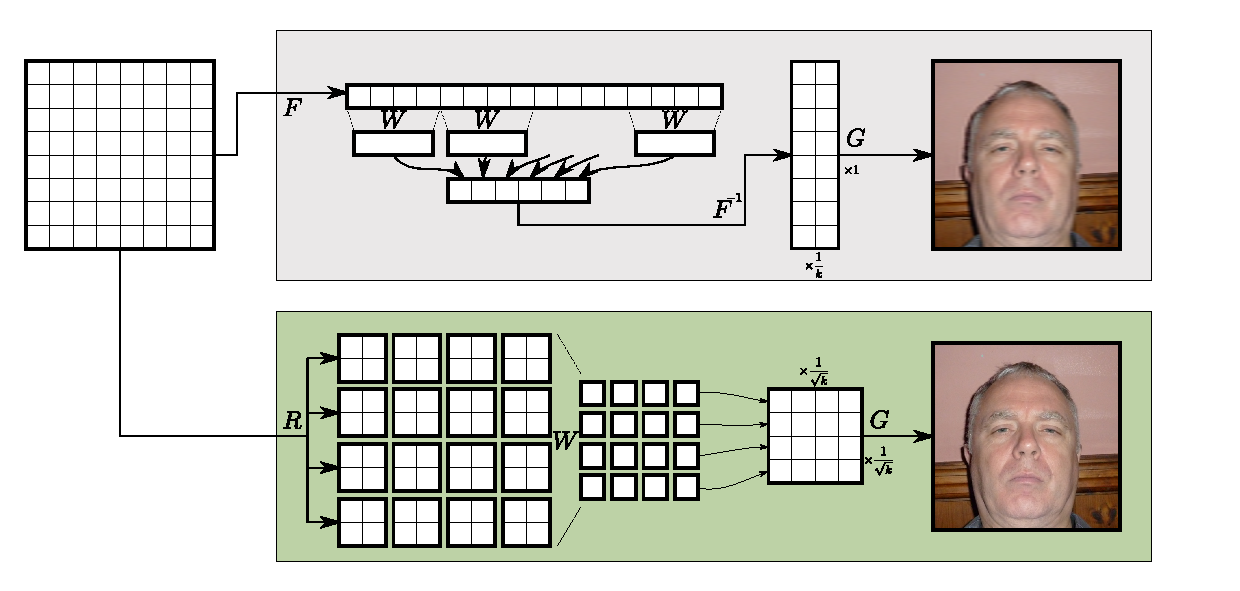
\includegraphics[width=\linewidth]{resample.pdf}
        \end{tikzfigure}
        \end{minipage}
        \hspace{-2cm}
        \begin{minipage}{0.25\linewidth}
            \Large
            %\vspace{0.5cm}
            \begin{itemize}
                \item[--] As a result of our work, we also found flaws in the
                    original formulation of hourglass transformers when used on
                    multi-dimensional data.
                \item[--] Our modifications have \textbf{applications in a wider
                    context}, outside of generative modelling.
            \end{itemize}
        \end{minipage}
        \end{tcolorbox}
    }

    \column{0.3}
    \block{}{
        \vspace{-1cm}
        \begin{tcolorbox}[boxsep=0pt,top=0cm,bottom=0.0cm,adjusted title={\huge\bf Results},colbacktitle=colorOne]
        \begin{tikzfigure}
            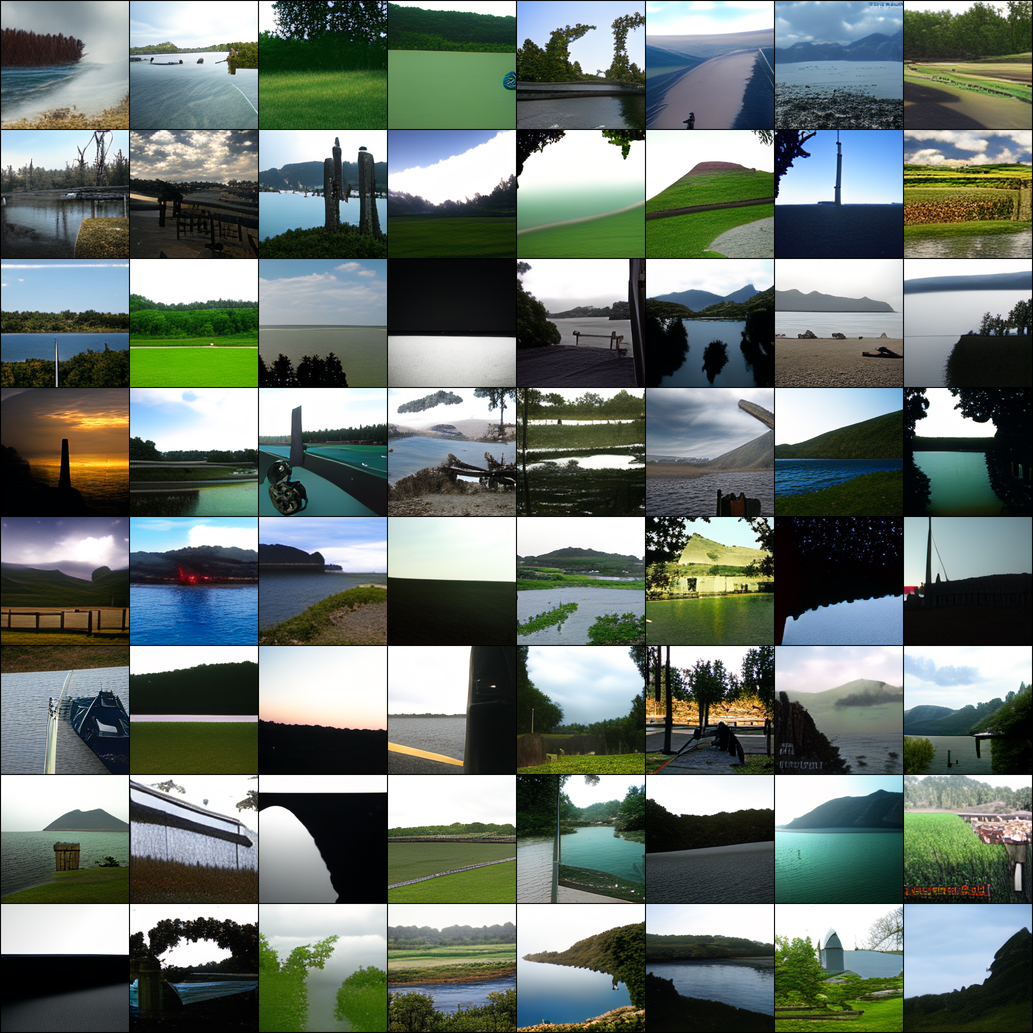
\includegraphics[width=0.49\linewidth]{imagenet-lakeside.png}
            \hfill
            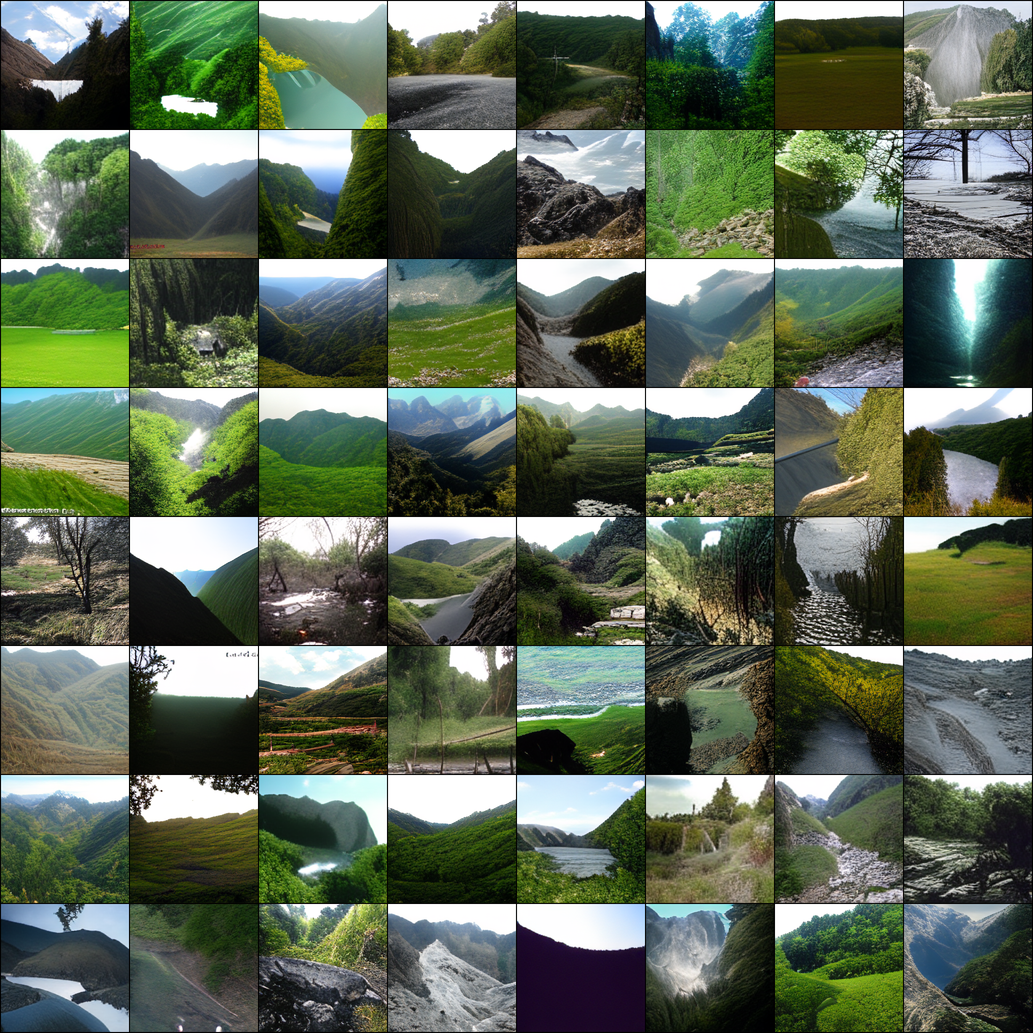
\includegraphics[width=0.49\linewidth]{imagenet-valley.png}
            %\captionof{figure}{
                %$256 \times 256$ class-conditioned samples on ImageNet. The left
                %batch of samples are from the class ``Lakeside'' whereas the
                %right batch are from the class ``Valley''. We note, that our
                %approach can be extended to use text prompts as a conditioning
                %signal, yielding a text-to-image model.
            %}
        \end{tikzfigure}
        \vspace{-0.5cm}
        {
            \Large
            \begin{itemize}
                \item[--] $256 \times 256$ \textbf{class-conditioned} samples from our
                    ImageNet model.
                \item[--] Left and right batches are from classes ``Lakeside''
                    and ``Valley'' respectively.
                \item[--] Our approach is easily extensible to use text prompts,
                    \textbf{yielding a fast text-to-image generator}.
            \end{itemize}
        }
        
        %\vspace{-1cm}

        \begin{tikzfigure}
            \includegraphics[width=0.49\linewidth]{inpaint-rand.png}
            \hfill
            \includegraphics[width=0.49\linewidth]{inpaint-block.png}
            %\captionof{figure}{
                %Representative inpainting results on FFHQ1024 using our trained
                %model. We demonstrate the superiority of NAR
                %methods for inpainting by using arbitrary inpainting masks,
                %including completely random (left) and large block masks
                %(right). Such patterns are difficult to inpaint with using 
                %autoregressive models, and cannot utilise the full context
                %available to them.
            %}
        \end{tikzfigure}
        \vspace{-0.5cm}
        {
            \Large
            \begin{itemize}
                \item[--] Example inpainting results using our FFHQ1024 model.
                    We show multiple results given the same image-mask pair to
                    \textbf{demonstrate diversity in the outputs}.
                \item[--] NAR methods allow for \textbf{arbitrary inpainting patterns} to
                    be easily used. In contrast, AR models cannot easily handle all
                    patterns, nor can they use all context when inpainting.
            \end{itemize}
        }
        \end{tcolorbox}
    }

    \block{}{
        \vspace{-1.5cm}
        \begin{tcolorbox}[boxsep=0pt,top=0cm,adjusted title={\huge\bf
            References},colbacktitle=colorOne]
        \nocite{*}
        \vspace{0.4cm}
        %\begin{footnotesize}
        \printbibliography[heading=none]
        %\end{footnotesize}
        \end{tcolorbox}
    }
\end{columns}
\end{document}
